% https://tex.stackexchange.com/q/570630/2891
% \documentclass[nols]{tufte-book}
\documentclass[]{tufte-book}
\usepackage{kantlipsum}
\usepackage{url}
\usepackage{graphicx}
\usepackage{csquotes}
\begin{document}
\title{Sample Document}
\author{Michal Hoftich}
\maketitle
\tableofcontents
\section{Introduction}

This is an example of Tufte \LaTeX\ document converted to Tufte HTML using \TeX4ht\footnote{\url{https://tug.org/tex4ht/}}.
It shows various commands provided by Tufte classes. Most of the text are just random words 
provided by the Kantlipsum\footnote{\url{https://ctan.org/pkg/kantlipsum?lang=en}} package, so please don't 
try to find a message in that.



\begin{marginfigure}
  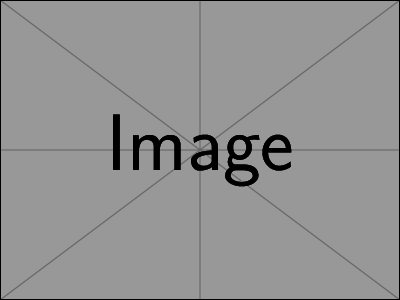
\includegraphics[width=\textwidth]{example-image.png}
  \caption{Example margin figure}
\end{marginfigure}

\section{First section}

Here is some math: \(a^2+b^2=c^2\)

\[e^{i\pi}+1=0\]

\kant[1]

\subsection{Hello, subsection}


\begin{figure}[tbt]
  \caption{Example figure}
  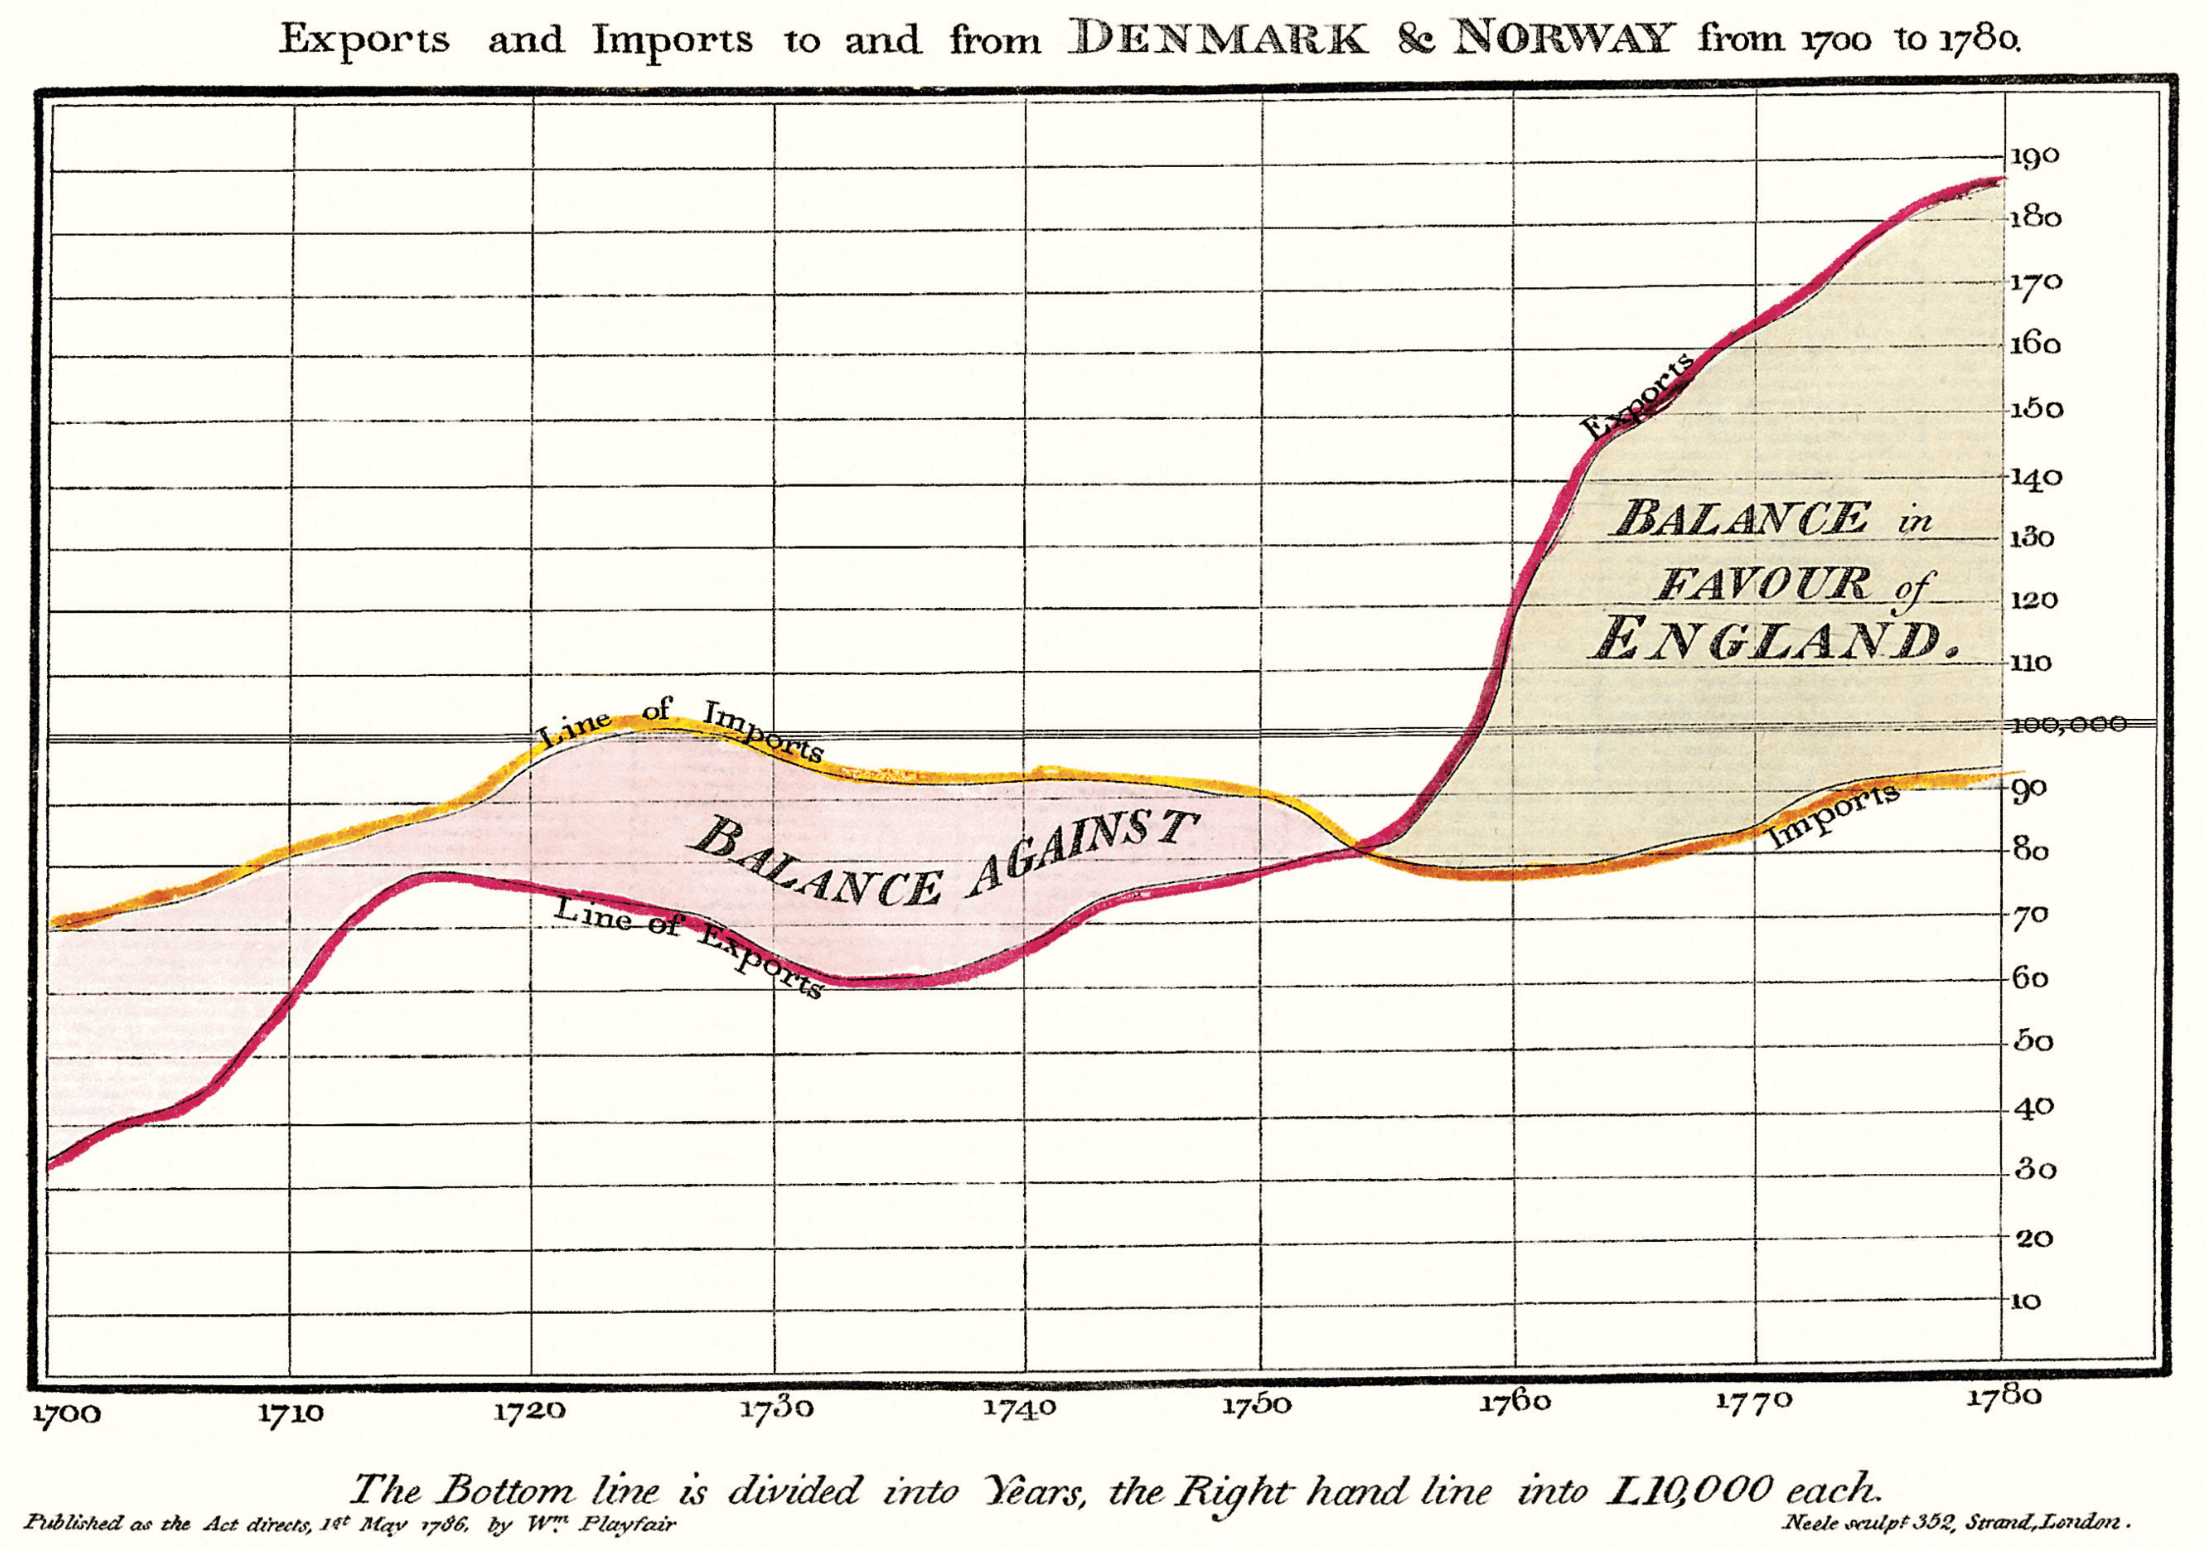
\includegraphics[width=\textwidth]{exports-imports.png}
\end{figure}

\kant[2]

\begin{displayquote}[Douglas Adams]
Parents of young organic life forms should be warned, that
towels can be harmful, if swallowed in large quantities.
\end{displayquote}

\begin{quote}
Parents of young organic life forms should be warned, that
towels can be harmful, if swallowed in large quantities.
\end{quote}

\blockquote[Douglas Adams]{%
Parents of young organic life forms should be warned, that
towels can be harmful, if swallowed in large quantities.
}

% margin tables don't work in HTML.
% \begin{margintable}
%   \begin{tabular}{l l}
%     hello & world\\
%     second & line
%   \end{tabular}
%   \caption{Margin table}
% \end{margintable}

\begin{figure*}[tbt]
  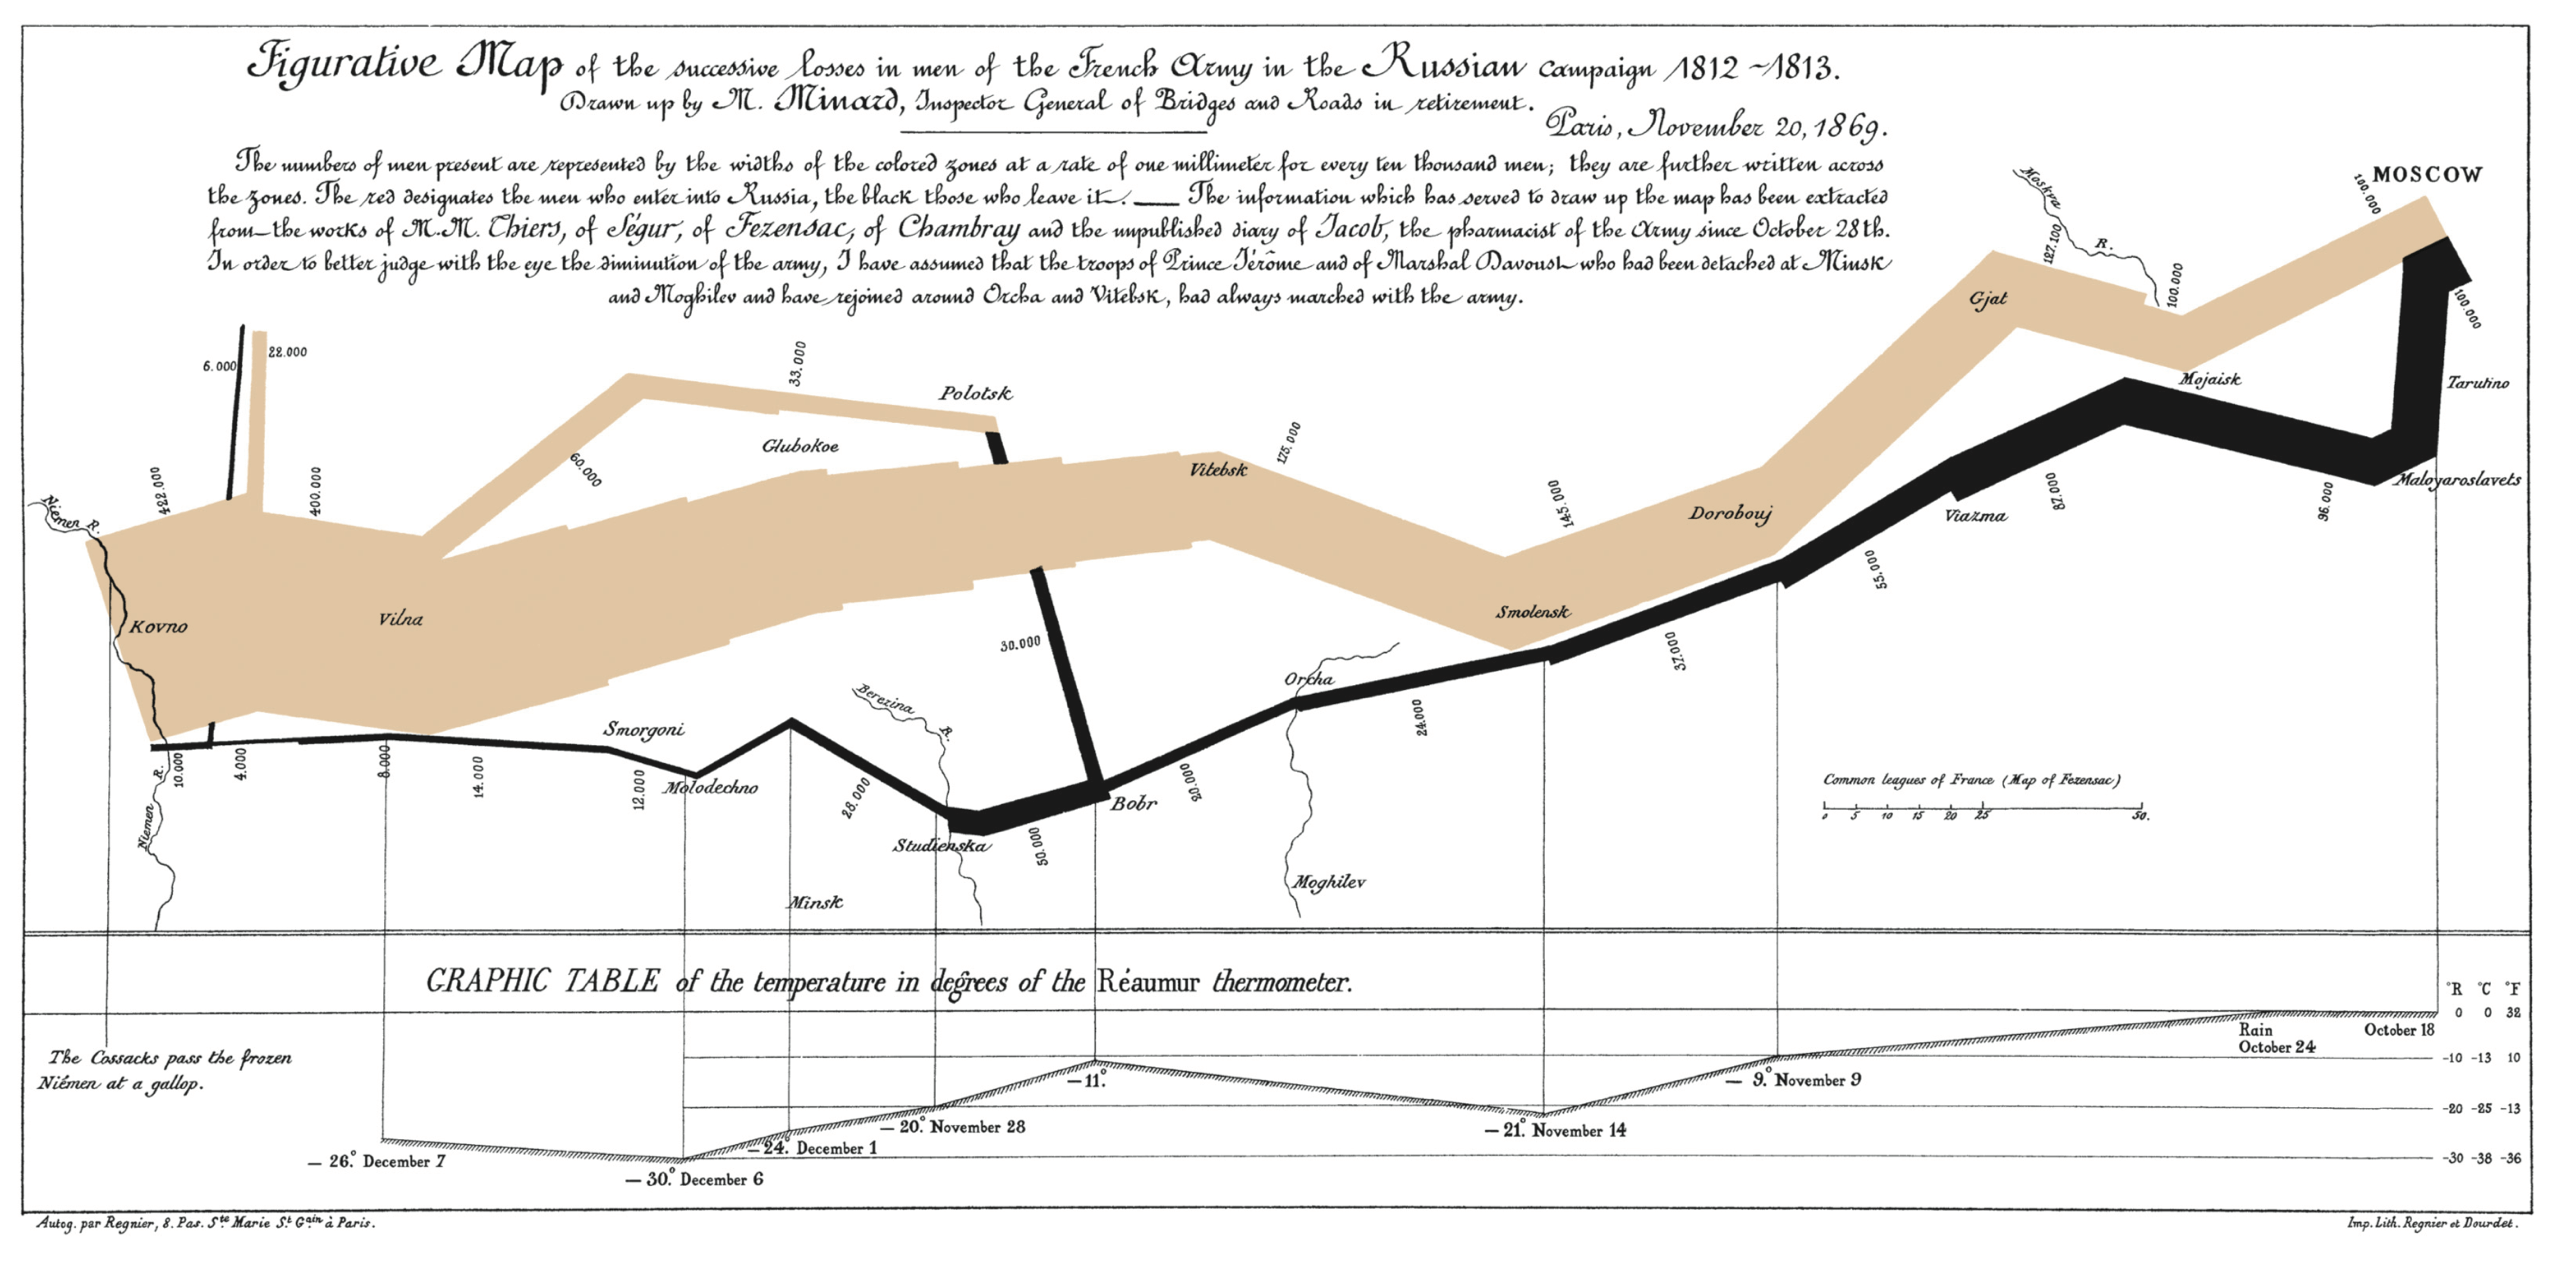
\includegraphics[width=\textwidth]{napoleons-march.png}
  \caption{Full width figure}
\end{figure*}
\begin{verbatim}
Hello verbatim 
Some special characters: {|}\ % "
\end{verbatim}

\newthought{We can try thought} \allcaps{uppercase} \textit{příliš žluťoučký kůň} \kant[3]

I am also interested in footnotes\footnote{Hello, this is a footnote}. \kant[4]

Another paragraph, try sidenote this time\sidenote{This is a sidenote}. And also marginnote\marginnote{Hello, this is a marginnote}.

I want to try citations\cite{Tufte2001,Tufte1990,Tufte1997,Tufte2006}.

\begin{fullwidth}
  This paragraphs is in full size \kant[5]
 \end{fullwidth}



\bibliography{sample-handout}
\bibliographystyle{plainnat}


\end{document}
